\section{Introduction}

Some datasets and simulators have been popularized lately among researchers in the probabilistic robotics field to handle tasks such as visual robot localization or the embodied question and answering problem\cite{DBLP:journals/corr/abs-1810-11181}. For instance, House3D\cite{YiHouse3D} is a virtual 3D environment containing 45000 indoor 3D scenes with any kind of 3D labeled objects. As another example, AI Habitat\cite{DBLP:journals/corr/abs-1904-01201} is a simulation platform for embodied AI agents training in a highly photorealistic and efficient 3D simulator. In this section Webots is presented as another simulator tool that can be used in the probabilistic robotics field. It offers the advantage to be highly customizable regarding to the robots and the world creation, it can be easily extended through custom robot windows plugins, and it is not oriented to visual robot localization only but any general robot localization task. 

Webots was created by Cyberbotics Ltd. a spin-off company from the EPFL. It has been developing it since 1998. The company currently\footnote{2019} employs 6 people in Lausanne, Switzerland to continuously develop Webots according to customers needs. Cyberbotics provides consulting on both industrial and academic research projects and delivers open-source software solutions to its customers. It also provides user support and training to the users of the Webots software. The source code and binary packages are available for free, their team provides support to the users through a Discord channel\footnote{\url{https://discordapp.com/invite/nTWbN9m}}. The program is available for MacOS, Ubuntu Linux, and Windows operative systems\cite{cyberbotics}.

Webots website has a reference manual that describes nodes and API functions. It has a complete user guide as well endowed with examples of simulations that show the use of actuators, creation of different environments, geometries primitives, complex behaviors, functionalities and advanced 3D rendering capabilities. This section is oriented to describe the basics of Webots and is focused on what will be useful to develop the project. For a detailed description please refer to the user guide\footnote{\url{https://cyberbotics.com/doc/guide/index}} or the reference manual\footnote{\url{https://cyberbotics.com/doc/reference/index}}.

For this project Webots R2020a version is used.

\section{Configuration of the Local Environment}

\subsection{Graphic Interface}
Webots supports the following programming languages: C, C++, Python, Java, MATLAB and ROS. Additionally, it offers the possibility of creating a custom interface to third-party software such as Lisp\textsuperscript{TM} or LabView\textsuperscript{TM} using TCP/IP protocol.

\begin{figure}[h]
	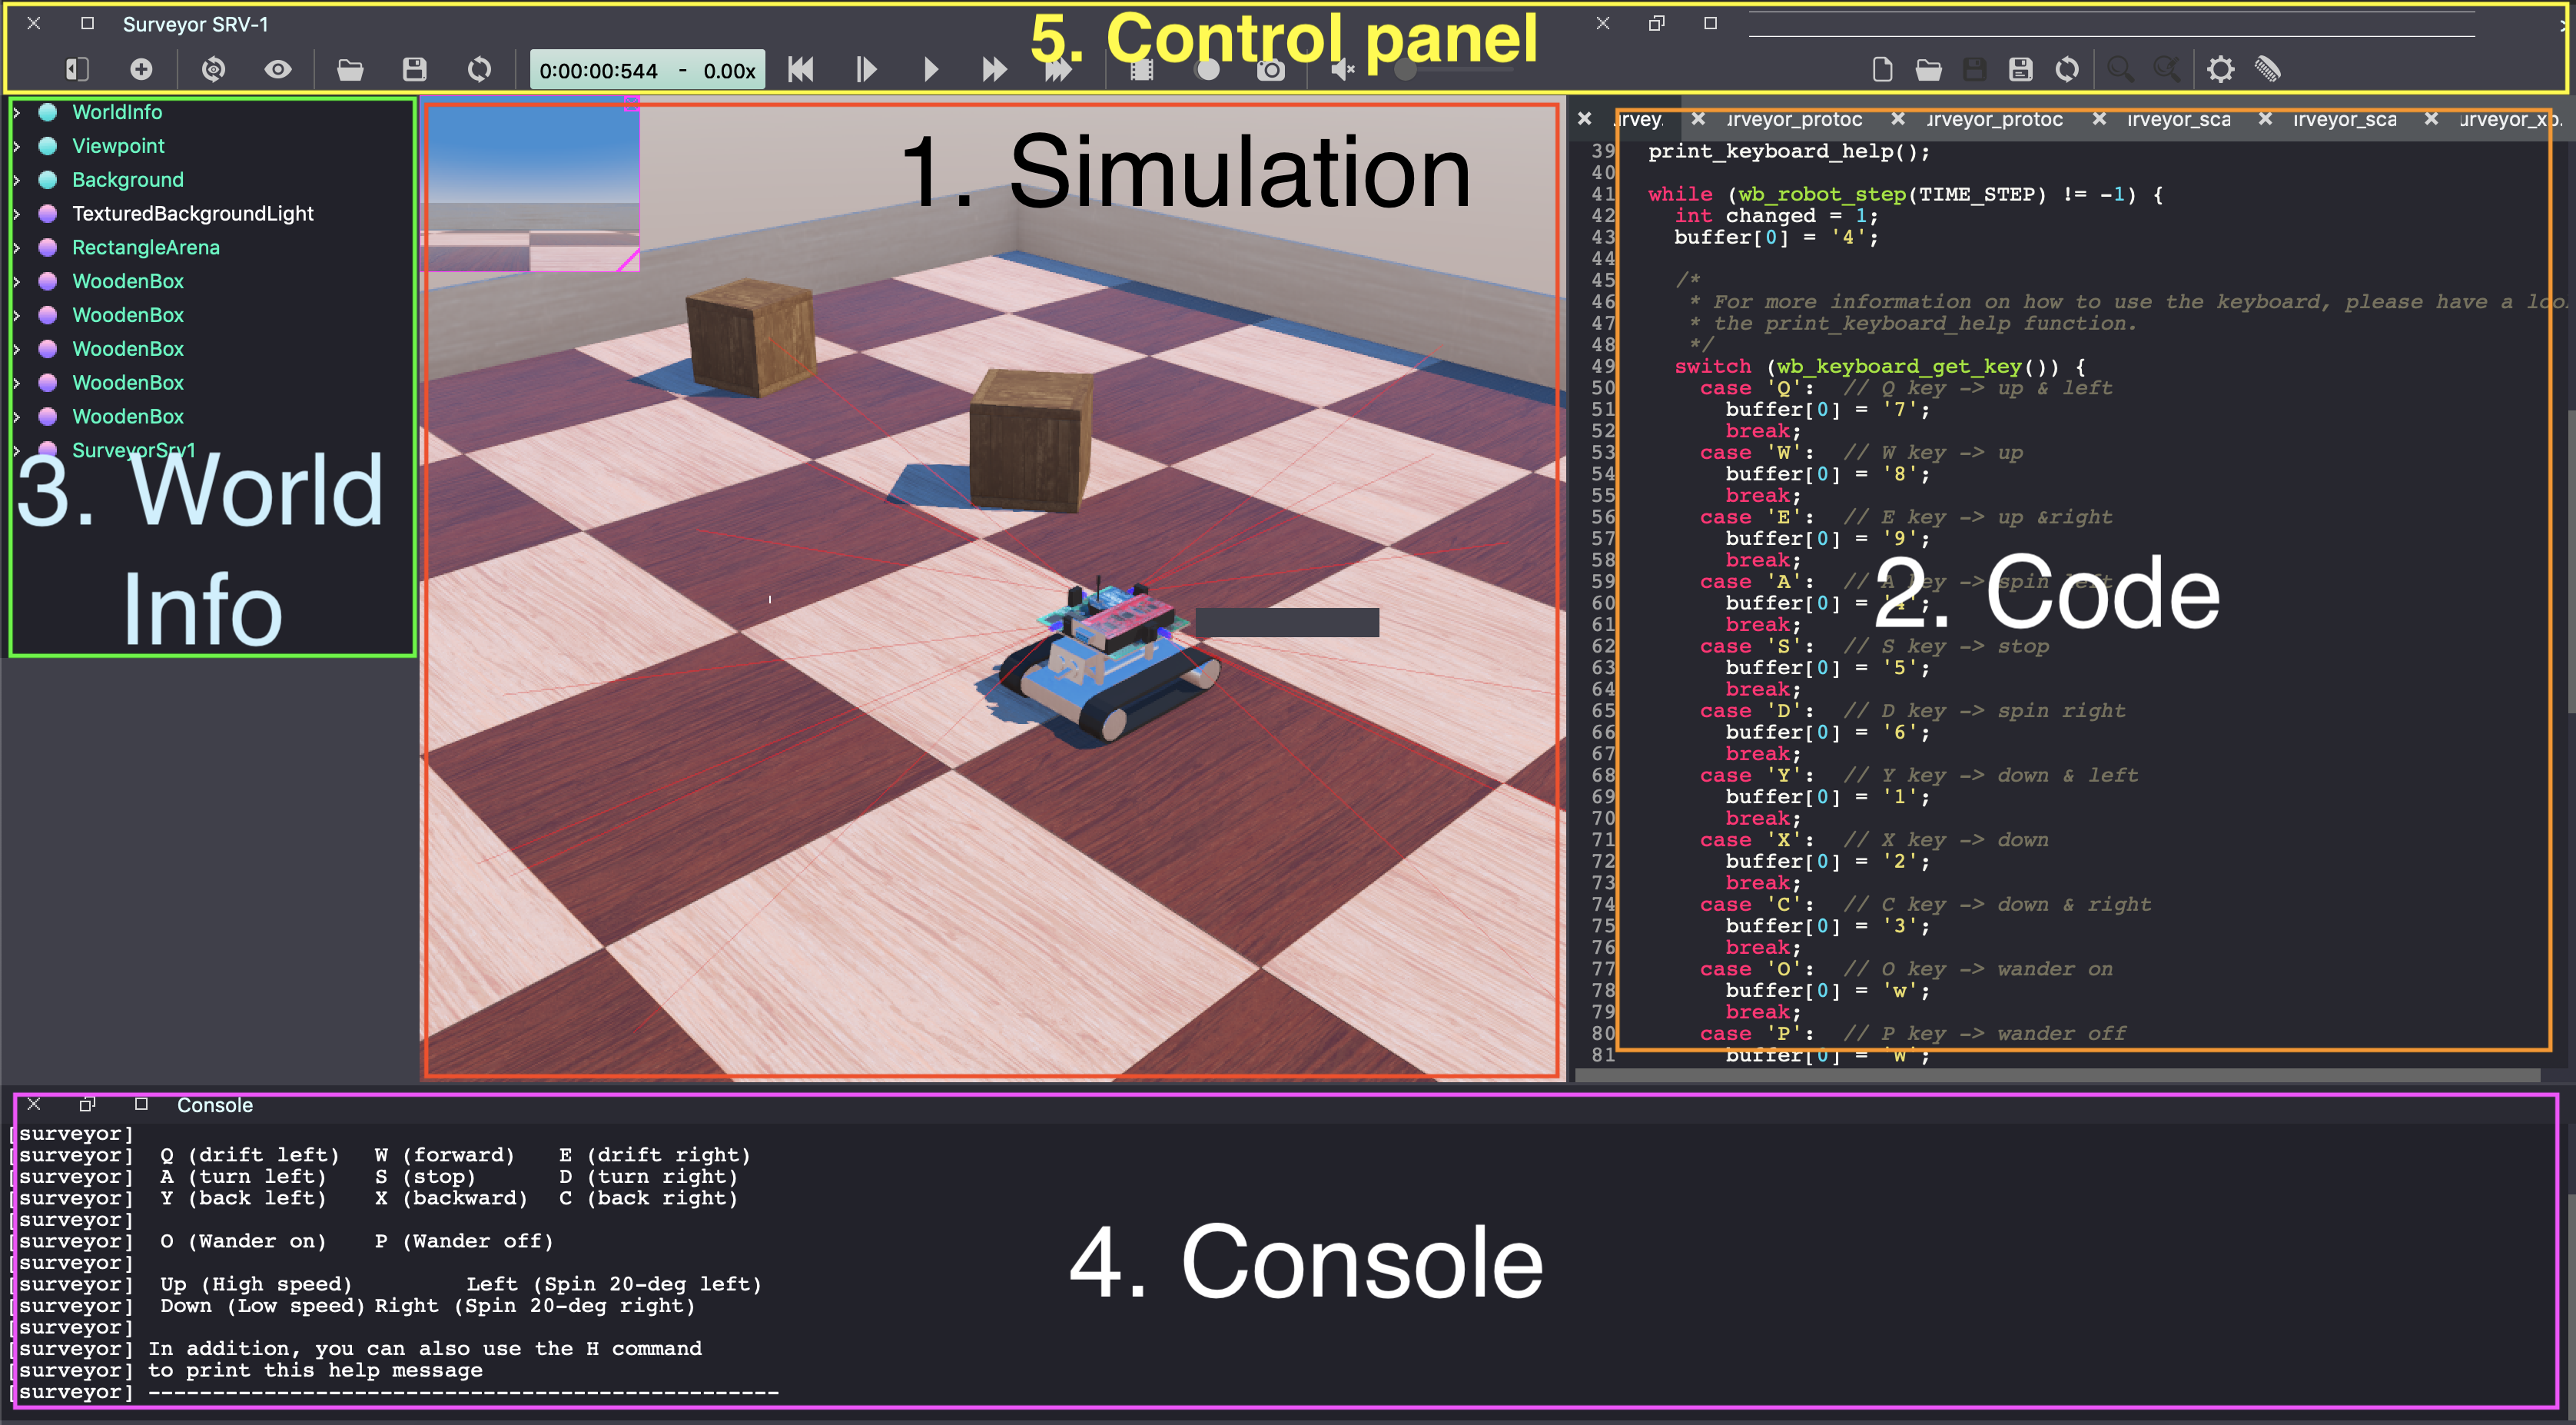
\includegraphics[width=\linewidth]{\images/chapter2/interface.png}
	\caption{Webots graphic interface}
	\label{fig-ch-2:interface}
\end{figure}

Figure \ref{fig-ch-2:interface} shows the main graphic interface of Webots. It can be divided in 5 panels:

\begin{enumerate}
	\item Simulation: graphic visualization of the simulated world objects.
	\item Code visualization: robot controller code editor.
	\item World Information: information represented in a tree structure about the simulated world including the robot components (sensors, actuators, physical characteristics), world objects, textures, etc. 
	\item Console: program execution output stream.
	\item Control panel: set of buttons that controls the simulation execution.
\end{enumerate}

The program allows users to create highly personalized simulated environments which are called worlds, from scratch using pre-built 3D object models such as robots, wood boxes, walls, arenas, etc. A robot needs to be associated with a controller program that contains the source code with the desired behavior. This controller can be easily edited in the code panel and once it is saved it is automatically reloaded into all the robots associated with it. For running the simulation, users can play, stop or reset it, among other options, using the control panel set of buttons. The output stream of the controller execution will be displayed in the console panel. 

\subsection{Webots with Python 3.7}

Python was created in 1990 by Guido van Rossum at Stichting Mathematisch Centrum in the Netherlands as a successor of a language called ABC\cite{python-docs}. Nowadays it has became one of the most popular programming languages for data science\cite{Raschka:2015:PML:2886323}.

The Python API of Webots was created from C++ API and it supports Python 3.7. It is possible to configure Webots to use Python 3.7 which should be previously installed from the Python website\footnote{Download it from \url{https://www.python.org}}; however, Webots does not work properly with Python versions installed from package managers as Brew. By default Webots is configured to use the default installed version of Python. In order to use another version, access to the menu options in Webots: \path{Webots/Preferences}; the \textit{Python command} label should point out to the installation path of Python3.7 as it is shown in figure \ref{fig-ch-2:python}. 

\begin{figure}[ht]
	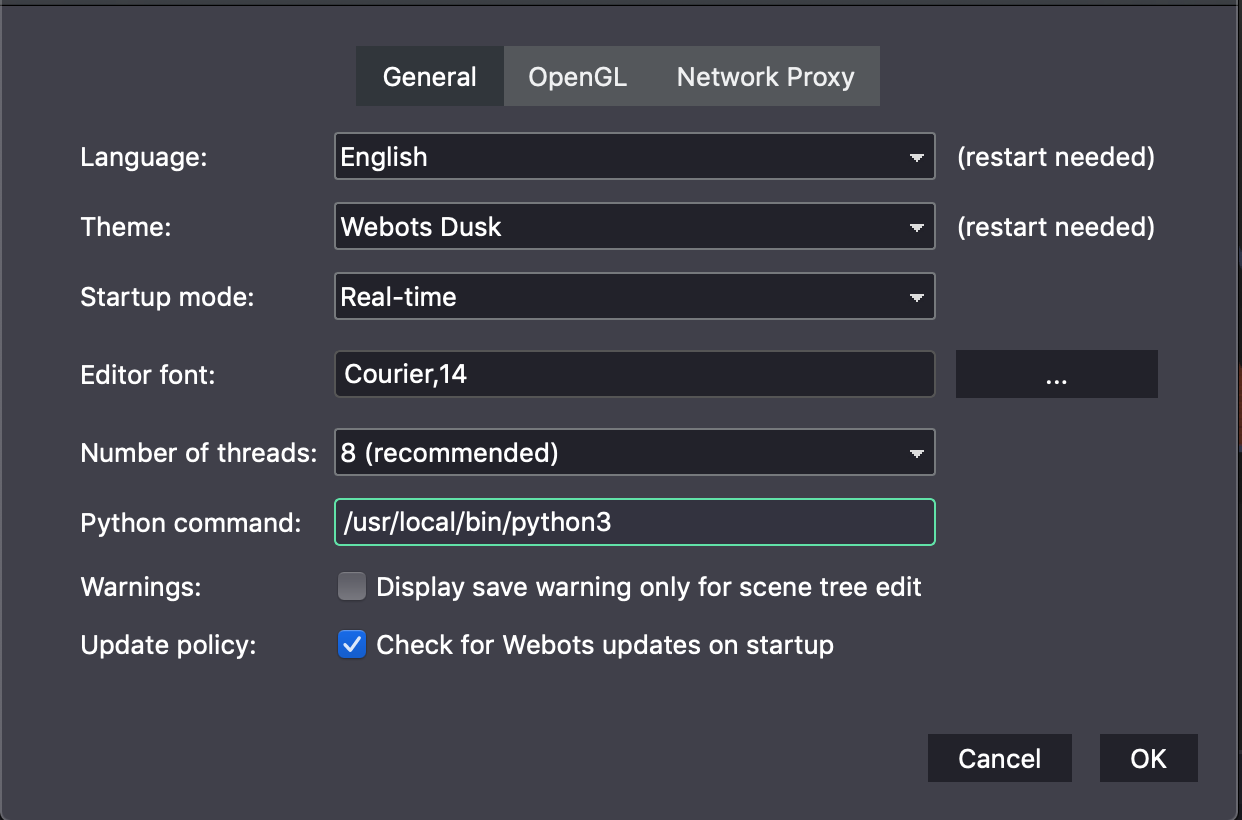
\includegraphics[width=\linewidth]{\images/chapter2/preferences.png}
	\caption{Configure Python3.7}
	\label{fig-ch-2:python}
\end{figure}

\subsection{Debug Controller}

When running a simulation is important to debug the code in order to catch some possible bugs on the program and to figure out why the program is not running as it should. Webots does not allow to debug code while running a simulation but it allows to run a robot controller from an external program such from an Integrated Development Environment (PyCharm, IntelliJ, Eclipse etc.), Python command lines, etc. This allows users to debug the controller. 

IntelliJ will be used as an example on how to configure an external controller to run the simulation on Webots using Python 3.7 code. 

The robot node has an option labeled \verb|controller| that specifies what controller the robot should use. This option should be configured selecting the \verb|<extern>| property as it is shown in figure \ref{fig-ch-3:external-controller}. This property tells Webots that the robot controller will be initiated using another application.

\begin{figure}[ht]
	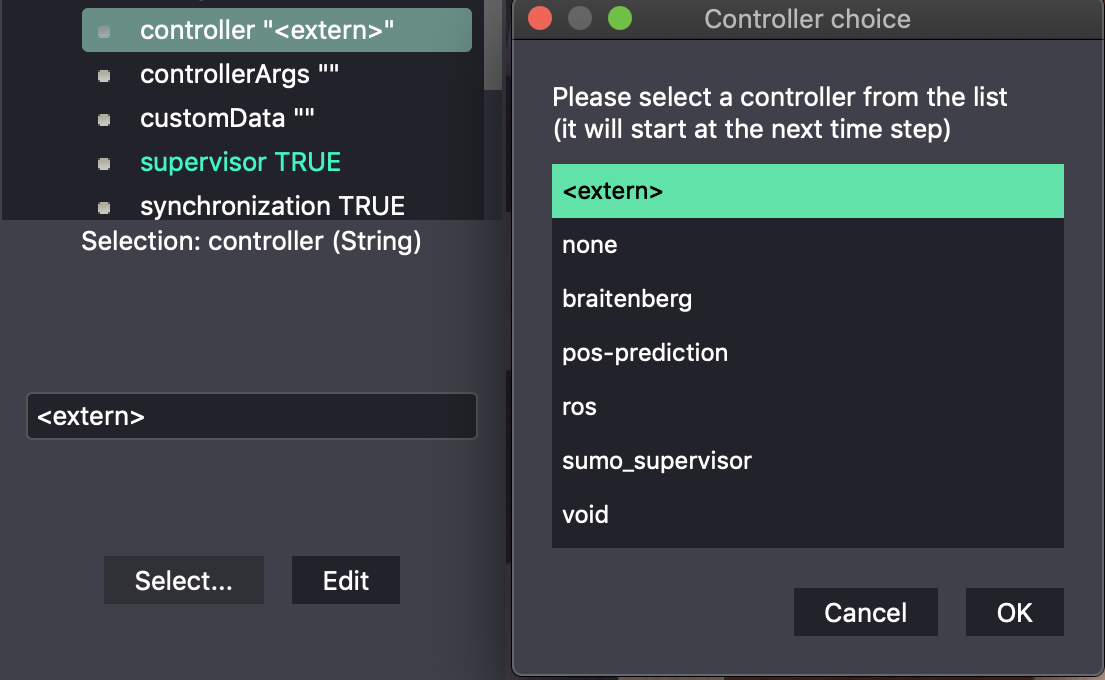
\includegraphics[width=\linewidth]{\images/chapter3/external-controller.png}
	\caption{Extern Controller in Webots}
	\label{fig-ch-3:external-controller}
\end{figure}

Table \ref{tab:ch-3:env-variables} show the environment variables needed to be configured for MacOS\footnote{For a complete list refer: \\ \url{https://cyberbotics.com/doc/guide/running-extern-robot-controllers?tab-os=macos&tab-language=python}}.

\begin{table}[]
\begin{tabular}{|l|l|}
\hline
\multicolumn{1}{|c|}{\textbf{Environment Variable}} & \multicolumn{1}{c|}{\textbf{Value}}            \\ \hline
\verb|WEBOTS_HOME|                                        & \verb|/Applications/Webots.app|                       \\ \hline
\verb|DYLD_LIBRARY_PATH|                                 & \verb|add ${WEBOTS_HOME}/lib/controller|          \\ \hline
\verb|PYTHONPATH|                                          & \verb|add ${WEBOTS_HOME}/lib/controller/python37| \\ \hline
\end{tabular}
\caption {Environment Variables Configuration for MacOS}
\label{tab:ch-3:env-variables}
\end{table}

In order to configure IntelliJ to use the Webots Python API a new project will be created, accessing to \verb|File/Project Structure.../Modules| and Add Content Root button can be used to add a new folder to the path, selecting the \verb|WEBOTS_HOME/lib/| \verb|controller/python37| folder as it is shown in figure \ref{fig-ch-3:add-content-root}.

\begin{figure}[ht]
	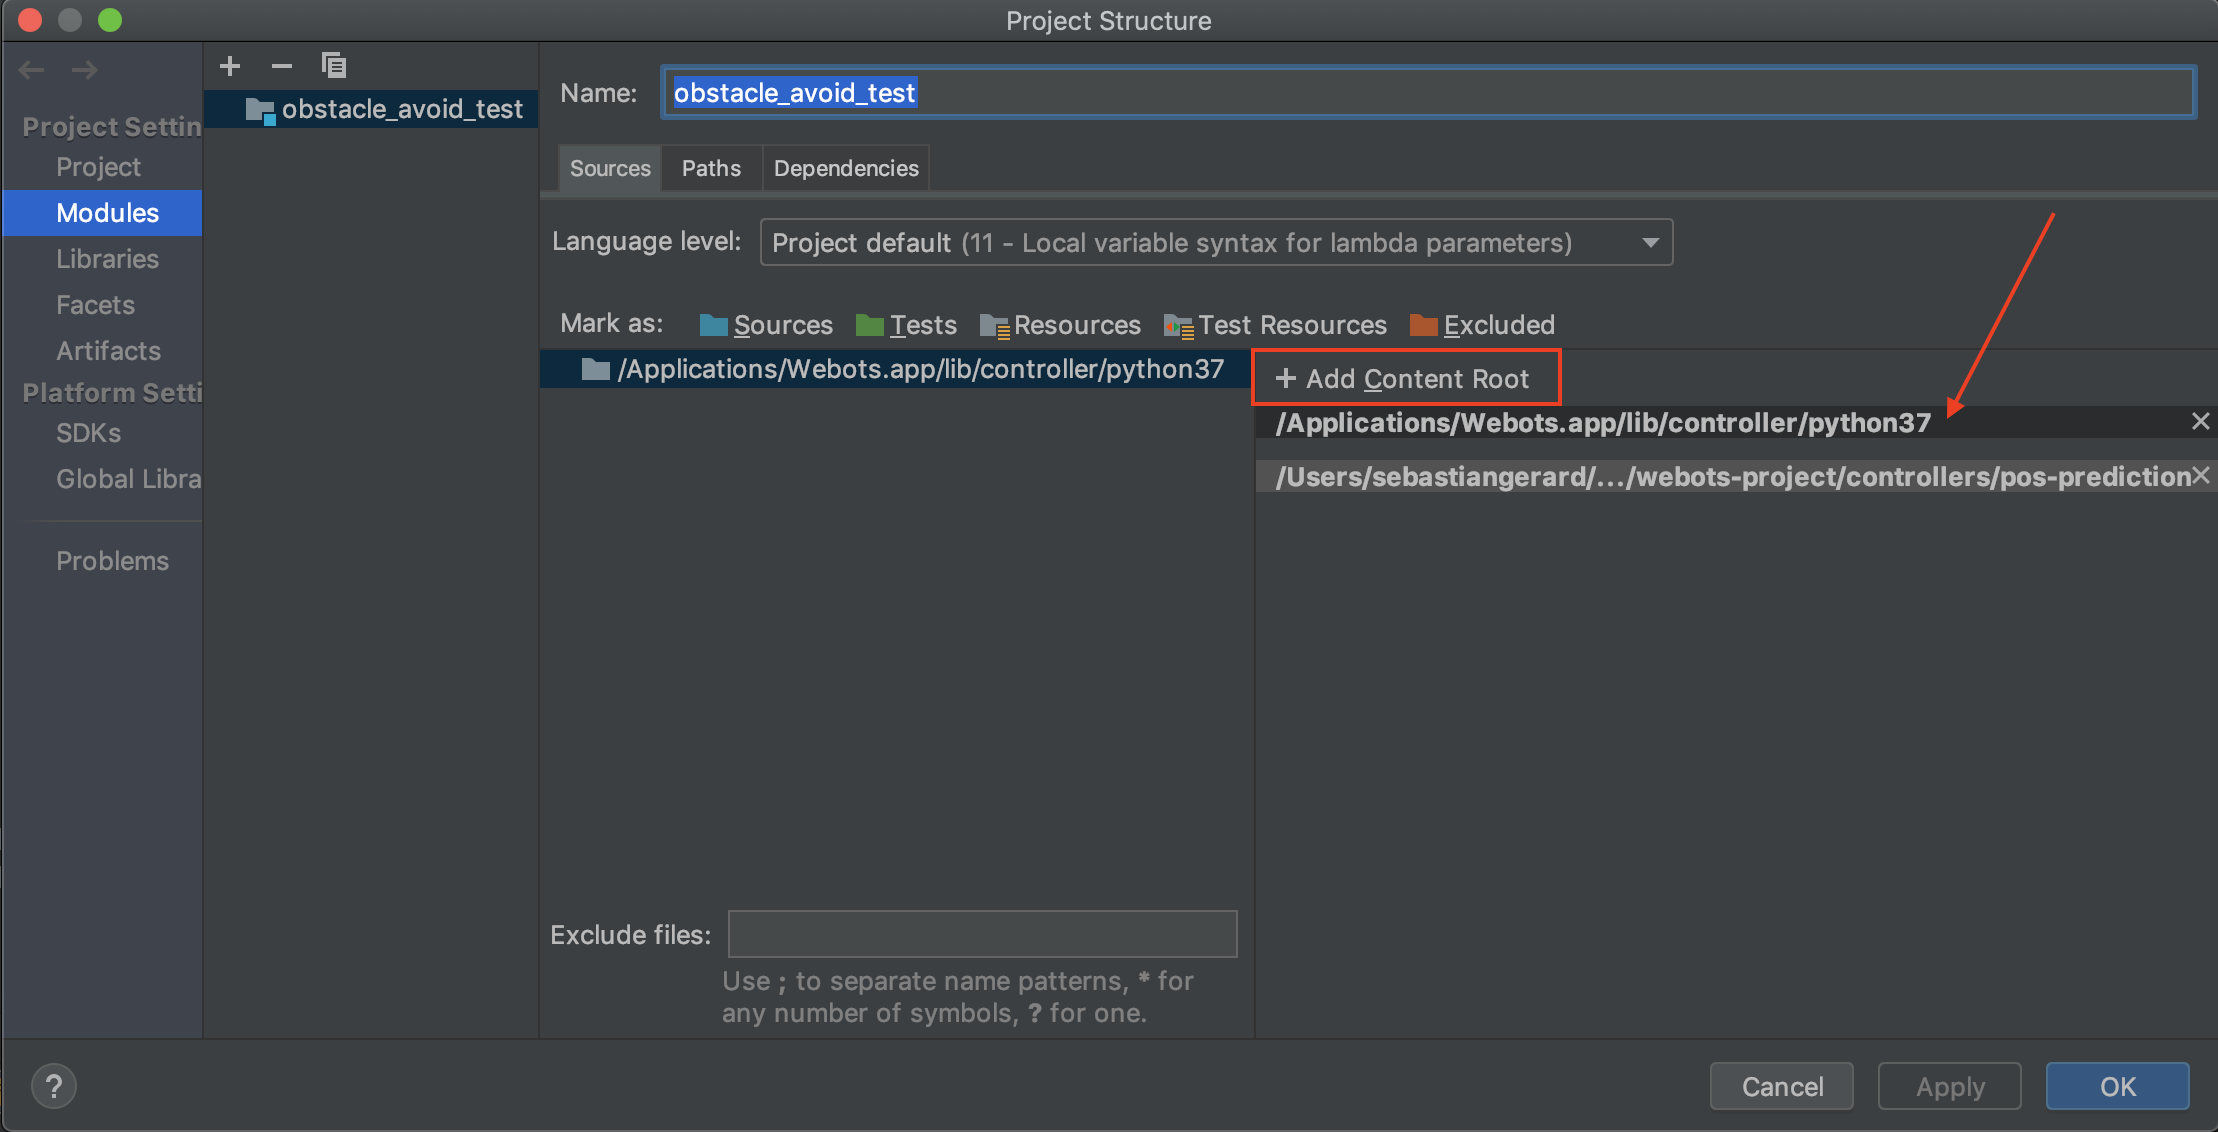
\includegraphics[width=\linewidth]{\images/chapter3/add-content-root.png}
	\caption{Extern Controller in Webots}
	\label{fig-ch-3:add-content-root}
\end{figure}

A final configuration is needed accessing to the menu option \verb|Run/Run...| then \verb|/Edit Configurations...|, and adding the needed environment variables as it is shown in figure \ref{fig-ch-3:params-ide}.

\begin{figure}[ht]
	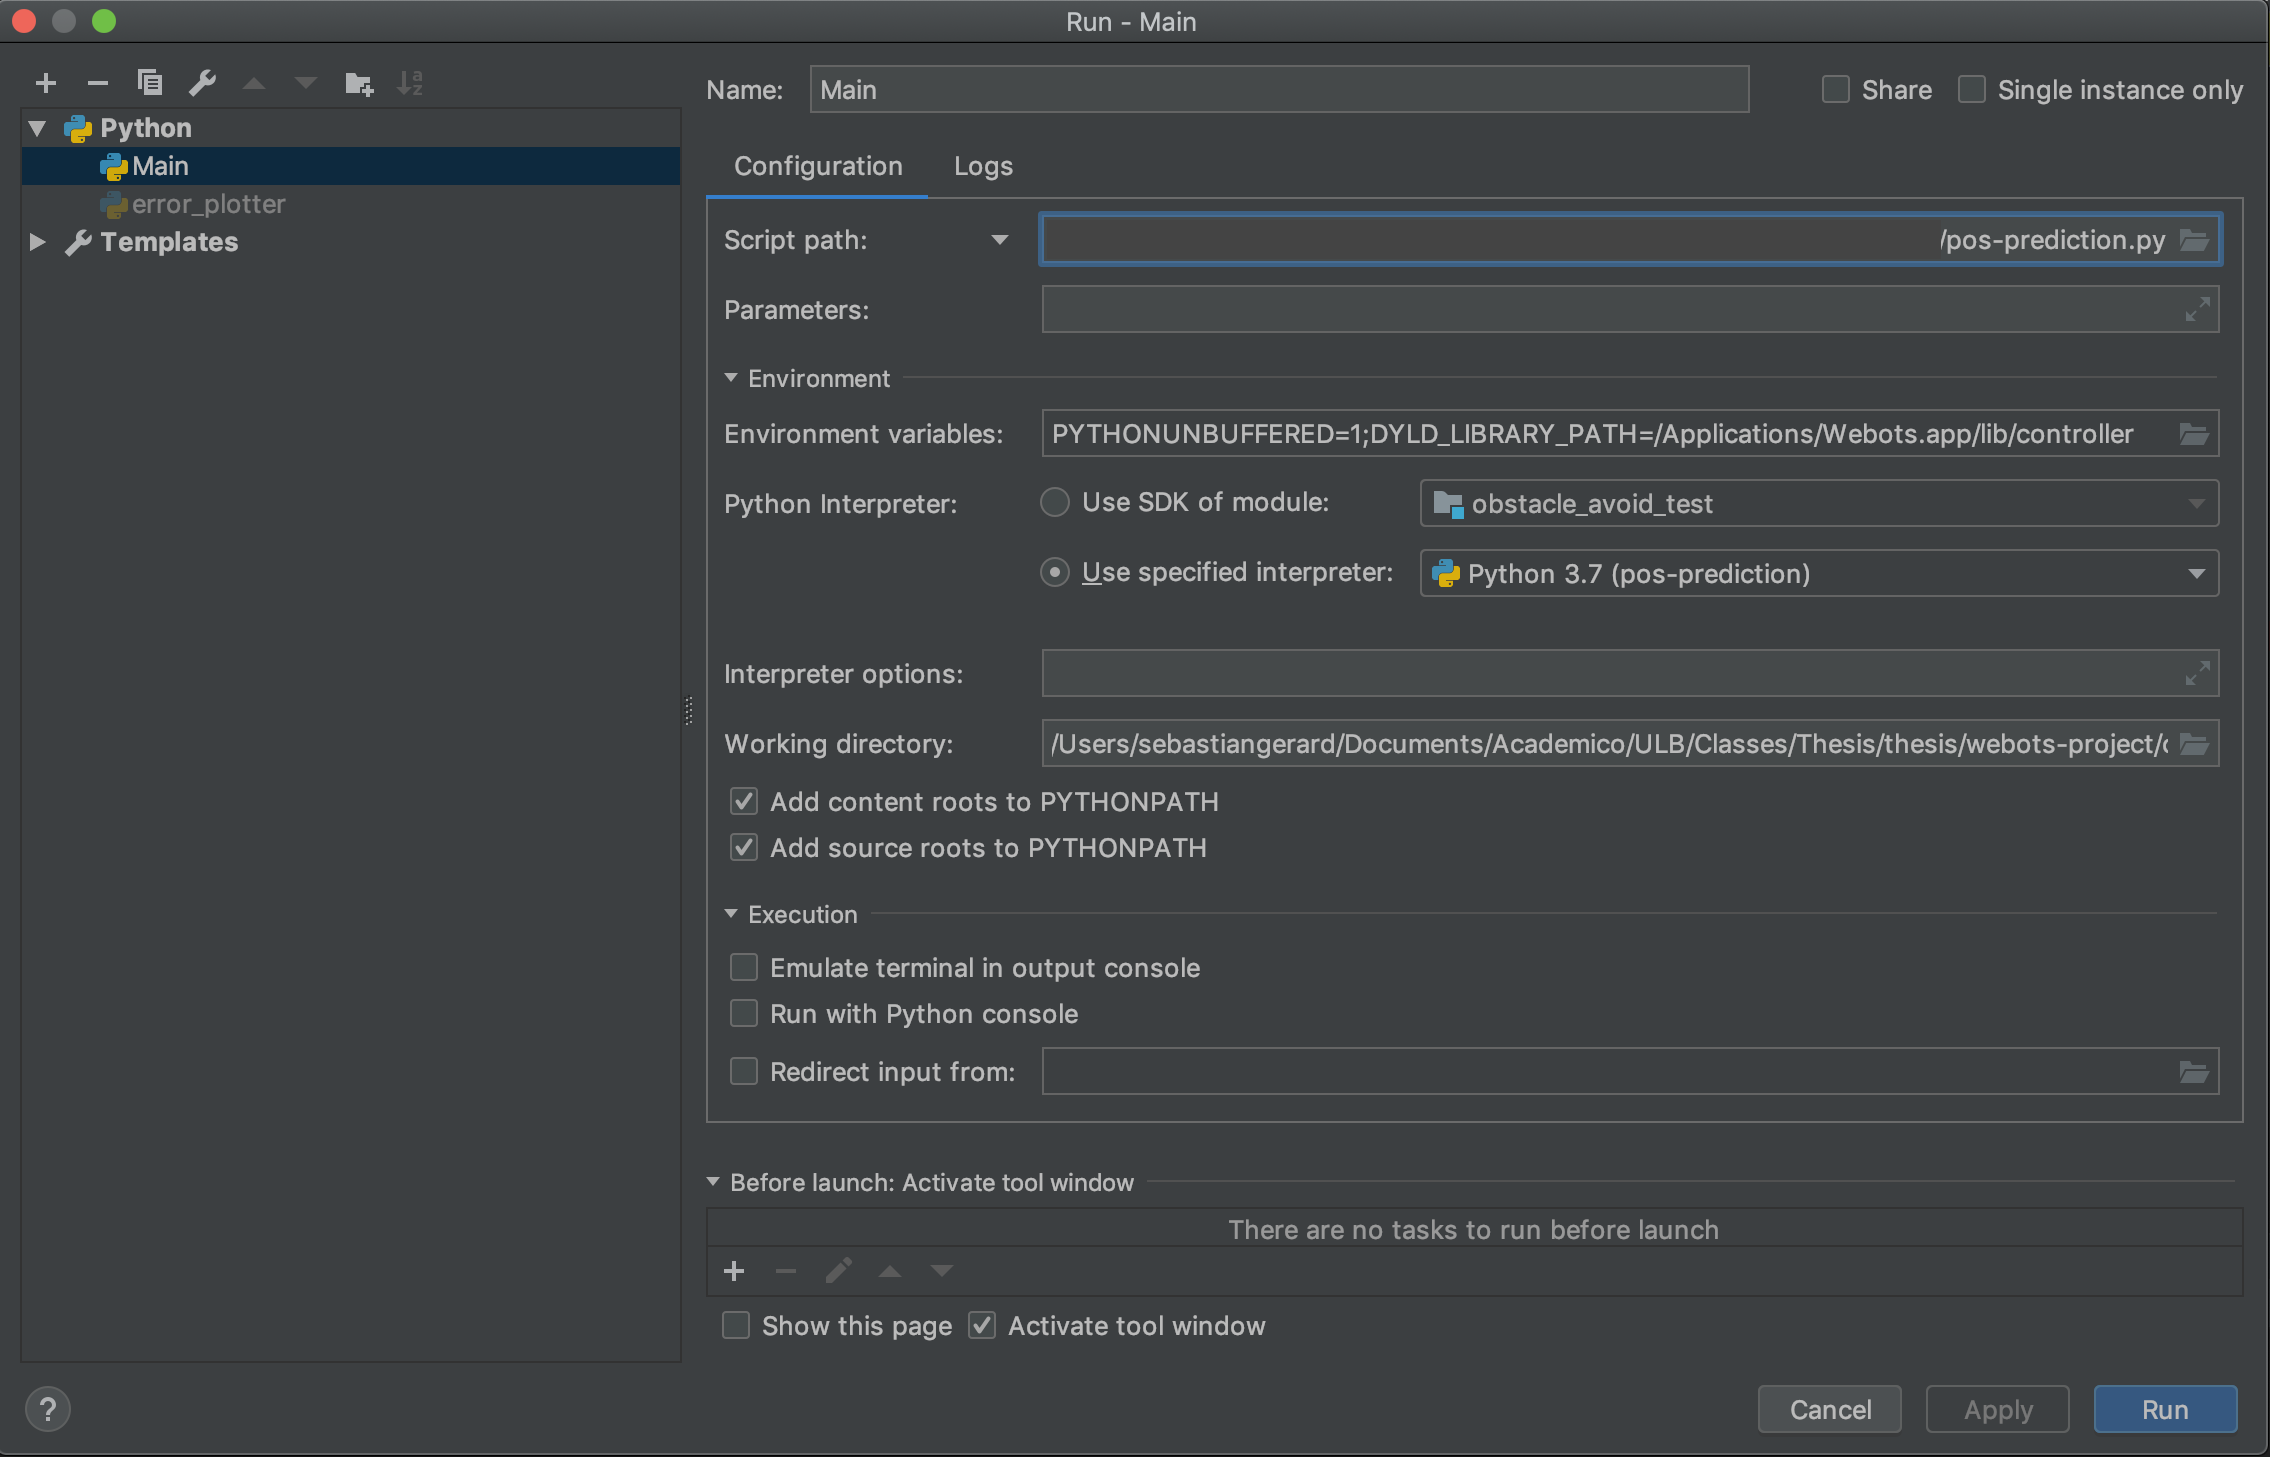
\includegraphics[width=\linewidth]{\images/chapter3/params-ide.png}
	\caption{Environment Variables Configuration IntelliJ}
	\label{fig-ch-3:params-ide}
\end{figure}

Once the configuration has been made IntelliJ is ready to run the controller. It can be made pressing on the \verb|Run| button. Debugging is also possible with the \verb|Debug| option.

\subsection{Install Python Libraries}

Installing the required python libraries for the project inside a python virtual environment is a good practice. To create a python virtual environment the command \verb|pip3 install virtualenv| can be used. 

The most-used libraries in this project are TensorFlow and Keras. 

TensorFlow is a Python-friendly open-source library developed by the researchers and engineers of the Google Brain team for internal use only and  then released in November 2015 under a permissive open source license. It implements machine learning algorithms and deep learning wrappers\cite{Raschka:2015:PML:2886323}.

The \verb|pip3| command allows to install any library for Python 3.7. For installing TensorFlow type \verb|pip3 install tensorflow| in the console terminal. For verifying the correct installation, the code displayed in listing \ref{code:verify-tf} can be put inside a controller application in Webots.

\begin{lstlisting}[language=Python, caption=Verify correct installation of TensorFlow, label=code:verify-tf]
import tensorflow as tf

verifier = tf.constant('TensorFlow was installed correctly.')
sess = tf.Session()
print(sess.run(verifier))
\end{lstlisting}

If TensorFlow is correctly installed, after the execution of the simulation, a message in the console panel will be displayed informing about its correct installation.

Keras is a high-level neural networks API, written in Python and capable of running on top of TensorFlow. It was developed with a focus on enabling fast experimentation\cite{kerasURL}. Similarly to TensorFlow, it can be installed using the \verb|pip3 install keras| command.

\section{Webots and the Virtual World}
Webots allows creating large simulated worlds. The world description and content is presented as a tree structure where each node represents an object in the world, those objects have themselves nodes and sub-nodes within a name and a value indicating different physical characteristics or components. 

\subsection{Robots and World Creation}

\begin{figure}[h!]
  \centering
  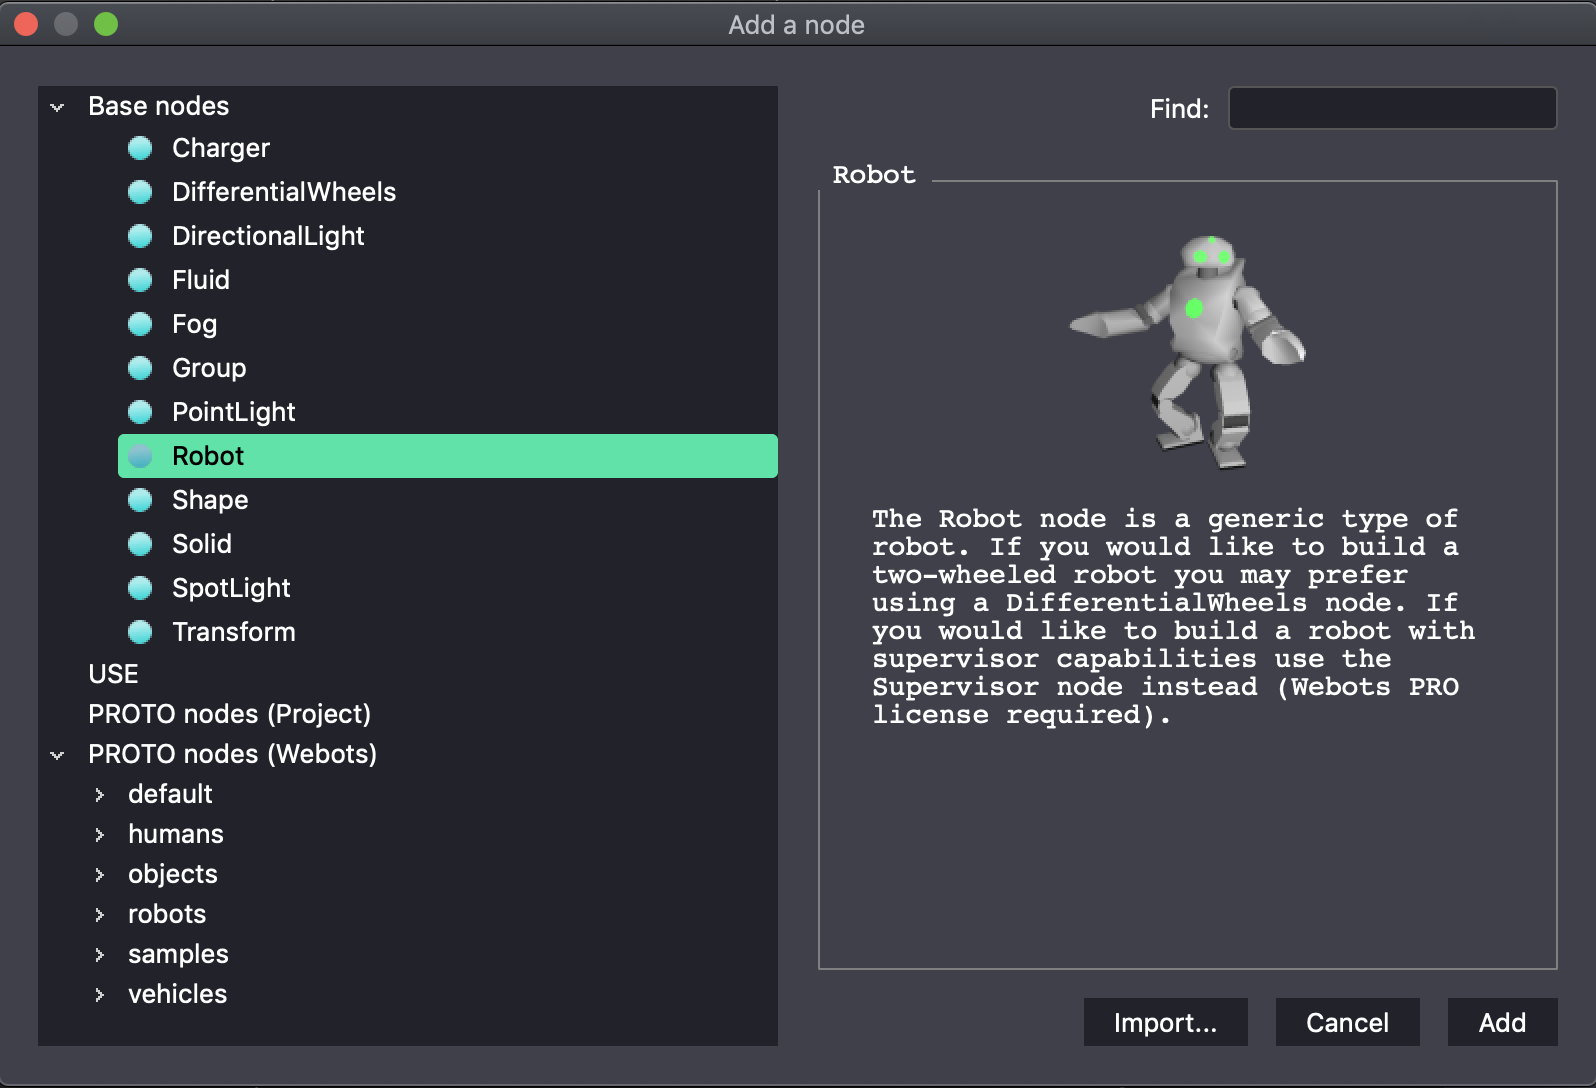
\includegraphics[width=0.8\linewidth]{\images/chapter2/nodes.png}
  \caption{World structure}
  \label{fig:ch-2:nodes}
\end{figure}

For adding a node into the world we can press the \verb|Add object| button that will open the window shown in figure \ref{fig:ch-2:nodes}. The base nodes are the basic objects that can be part of the world. Moreover, they are simpler models than the others. The USE nodes are objects that were already created in the world and can be reused. For instance, if a wood box was added into the world with some specific physical characteristics, a name can be assigned to its USE attribute and then it can be reused instead of creating a new one with same characteristics. The PROTO nodes contains a set of 3D models as robots, objects, vehicles, etc. Fruits, toys, drinks, plants, chairs, stairs and buildings are only a small part of the big set of modeled objects. The robots node offers as well a big diversity of models. From simple robots as the e-puck (figure \ref{fig:ch-2:e-puck}) model which is used very often in research, to more complex robots as the very well known humanoid Nao (figure \ref{fig:ch-2:nao}) are some examples of a total of 44 3D modeled robots that are available to use within the simulator tool. 

\begin{figure}[h!]
  \centering
  \begin{subfigure}[b]{0.3\linewidth}
  	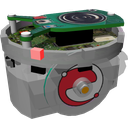
\includegraphics[width=\linewidth]{\images/chapter2/e-puck.png}
  	\caption{e-puck}
  	\label{fig:ch-2:e-puck}
  \end{subfigure}
  \begin{subfigure}[b]{0.35\linewidth}
  	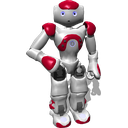
\includegraphics[width=\linewidth]{\images/chapter2/nao.png}
  	\caption{Nao}
  	\label{fig:ch-2:nao}
  \end{subfigure}
  \caption{Robots}
\end{figure}

Another powerful feature of Webots is to create a custom robot model from scratch using a tree-based structure of solid nodes which are virtual objects with physical properties. Thus a robot is made of a set of solid nodes put them together using joint nodes which are abstract nodes that models mechanical joints. Figure \ref{fig:ch-2:joints} shows the different types of joints that can be used.

\begin{figure}[h!]
  \centering
  \begin{subfigure}[b]{0.47\linewidth}
  	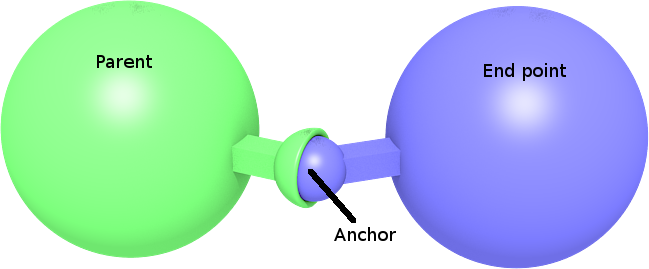
\includegraphics[width=\linewidth]{\images/chapter2/ballJoint.png}
  	\caption{Ball Joint}
  	\label{fig:ch-2:ball-joint}
  \end{subfigure}
  \vspace{0.00mm}
  \begin{subfigure}[b]{0.47\linewidth}
  	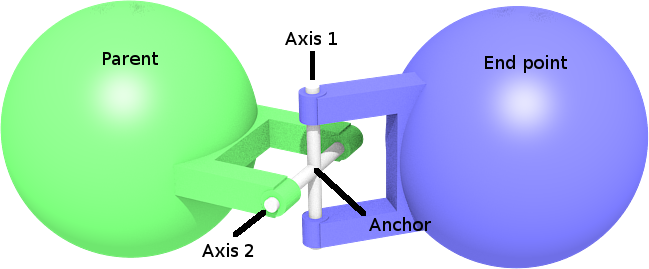
\includegraphics[width=\linewidth]{\images/chapter2/hinge2Joint.png}
  	\caption{Hinge 2 Joint}
  	\label{fig:ch-2:highe-2-joint}
  \end{subfigure}
  \vspace{0.00mm}
  \begin{subfigure}[b]{0.47\linewidth}
  	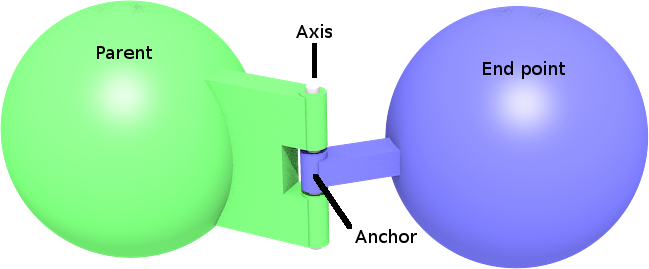
\includegraphics[width=\linewidth]{\images/chapter2/hingeJoint.png}
  	\caption{Hinge Joint}
  	\label{fig:ch-2:hinge-joint}
  \end{subfigure}
  \vspace{0.00mm}
  \begin{subfigure}[b]{0.47\linewidth}
  	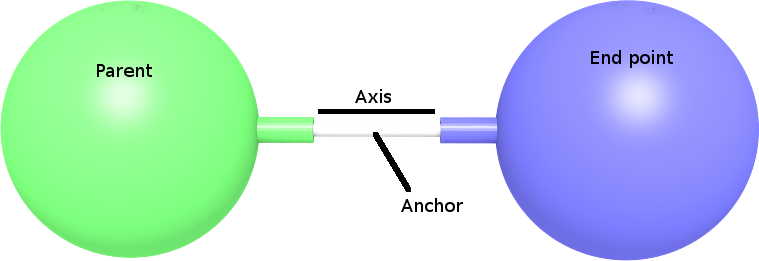
\includegraphics[width=\linewidth]{\images/chapter2/sliderJoint.png}
  	\caption{Slider Joint}
  	\label{fig:ch-2:slider-joint}
  \end{subfigure}
  \caption{Different types of joint nodes}
  \source{Webots documentation}
  \label{fig:ch-2:joints}
\end{figure}


A position sensor can be added into the devices property of a joint node in order to monitor it. In like manner a rotational motor node can be added for actuating it. Thus, putting all together a simplistic version of a custom robot can be created based on the tree information and properties given to the simulator.

\subsection{Sensors}\label{sec:ch-2:sensors}

Sensors allows the robot to sense the environment. Webots has a wide range of generic and commercially available sensors that can be plugged into a custom robot. On one side, the compass, distance sensor and position sensor are some few examples of generic sensors. On the other side, camera, lidar, radar and range finder sensors built by different manufacturers as Hokuyo, Velodyne and Microsoft are offered as subcategories of commercially available sensors. 

\begin{itemize}
\item{The \textbf{compass sensor} can be used to express the angle orientation of the robot over the position of the virtual north as a 1, 2 or 3-axis vector (roll, pitch and yaw angles). The virtual north can be specified in the WorldInfo node by the \verb|northDirection| field. The major fields that can be customized are: the xAxis, yAxis, zAxis, lookup table and resolution field. }
\item{The \textbf{distance sensor} measures the distance between the sensor and an object throughout rays collision with objects. Webots models different types of distance sensors as: generic, infra-red, sonar and laser. All of these has a lookup table, number of rays cast by the sensor, aperture angle, gaussian width and resolution field that can be personalized according to the needs.}
\item{A \textbf{position sensor} can be inserted into the device field of a Joint or a Track. It measures the mechanical joint position. Moreover, the noise and resolution of the sensor can be customized. This sensor is useful for estimating the position of a robot given the current position of a mechanical joint, this technique is known as Odometry.}
\end{itemize}

\begin{figure}[h!]
  \centering
  \begin{subfigure}[b]{0.3\linewidth}
  	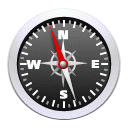
\includegraphics[width=\linewidth]{\images/chapter2/compass.png}
  	\caption{Compass sensor}
  	\label{fig:ch-2:compass}
  \end{subfigure}
  \vspace{0.00mm}
  \begin{subfigure}[b]{0.3\linewidth}
  	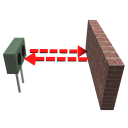
\includegraphics[width=\linewidth]{\images/chapter2/distance-sensor.png}
  	\caption{Distance sensor}
  	\label{fig:ch-2:distance-sensor}
  \end{subfigure}
  \vspace{0.00mm}
  \begin{subfigure}[b]{0.3\linewidth}
  	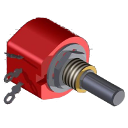
\includegraphics[width=\linewidth]{\images/chapter2/position-sensor.png}
  	\caption{Position sensor}
  	\label{fig:ch-2:position-sensor}
  \end{subfigure}
  \vspace{0.00mm}
  \caption{Sensors}
  \source{Webots documentation}
  \label{fig:ch-2:sensors}
\end{figure}

Sensors have some fields in common. For instance, the resolution field that indicates the sensitivity of the measurement. When it is set to -1 means that it will measure the infinitesimal smallest perceived change. As another example, the lookup table is a field that maps a value from the sensor read data to another custom value. Additionally, the standard deviation noise introduced by the sensor can be specified for a given measure. 

Table \ref{tab:ch-2:lookup} shows the possible values that can be associated with the lookup table field. The first column represents the data measured by the sensor, the second column is the mapped value and the third column represents the noise as a gaussian random number whose range is calculated as a percentage of the response value\cite{cyberbotics}. For instance, for the row $[0.3, 50, 0.1]$ when the sensor senses an object to 0.3m of distance from the robot, it will return a value of $50 \pm 5$, where 5 represents the standard deviation, that is the $10\%$ of 50.
\begin{table}[h!]
\centering
 \begin{tabular}{c c c} 
 \hline
 Value & Mapped value & Noise \\ [0.5ex] 
 \hline\hline
 0 & 1000 & 0 \\ 
 \hline
0.1 & 1000 & 0.1 \\ 
 \hline
 0.2 & 400 & 0.1 \\ 
 \hline
 0.3 & 50 & 0.1 \\ 
 \hline
 0.37 & 30 & 0 \\ 
 \hline
\end{tabular}
\caption{Lookup table of distance sensor}
\source{Webots documentation}
\label{tab:ch-2:lookup}
\end{table}

Figure \ref{fig:ch-2:lookup} shows the relation between the current sensor values and the mapped values within the associated noise.

\begin{figure}[h!]
  \centering
  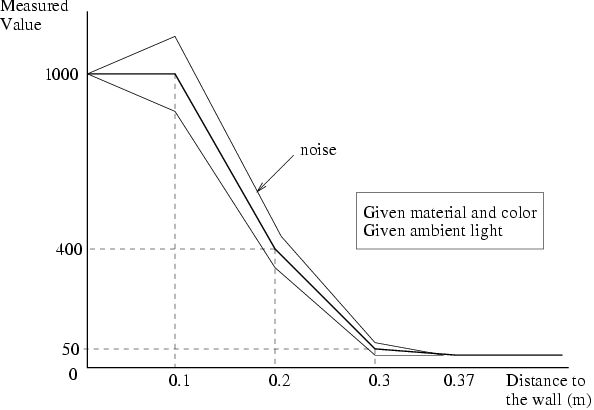
\includegraphics[width=0.8\linewidth]{\images/chapter2/lookuptable.png}
  \caption{Sensor response versus obstacle distance}
  \source{Webots documentation}
  \label{fig:ch-2:lookup}
\end{figure}

\subsection{Actuators}

Actuators allows the robot to modify the environment. Webots can simulate rotational motors, linear motors, speakers, LEDs, etc. 

\section{Webots Controller Plugins}

Webots allows the creation of custom user-implemented windows interfaces for the robots which are integrated to Webots using a controller plugin. 

\subsection{Robot Window}

A robot window is a custom window that can be made using HTML and Javascript and then associated to a specific robot using its \verb|window| property. The robot windows need to be created under the \verb|plugin/robot_windows/<window_name}>| directory. The window's name should be the same as the controller's name; otherwise, Webots does not recognize it and therefore it does not display it under the windows list.

The controller can send and receive messages to the window robot using the command \verb|wwiSendText(text)| and \verb|wwiReceiveText()| respectively. Similarly the window robot can communicate with the controller with the \verb|webots.window(" <window| \verb|name> ").receive| and \verb|webots.window(" <window name> ").send| commands. 

\begin{figure}[h!]
  \centering
  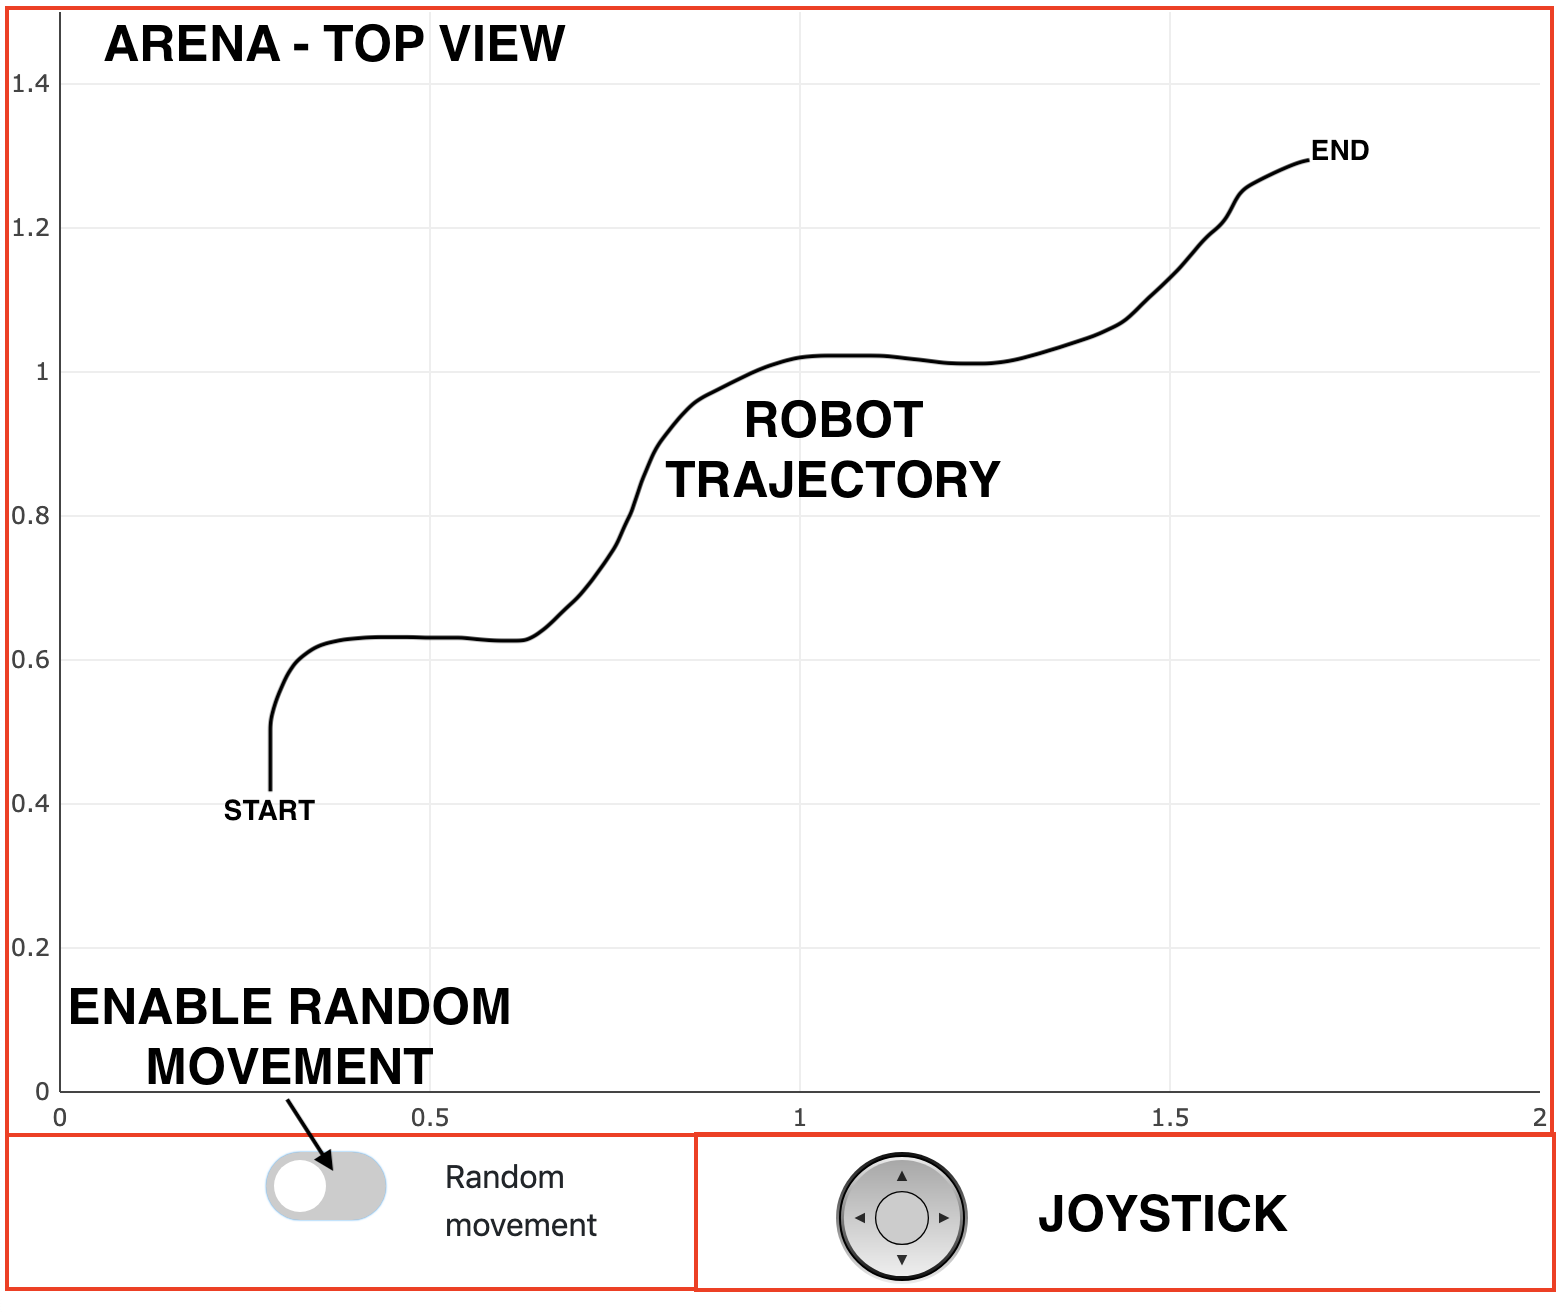
\includegraphics[width=0.8\linewidth]{\images/chapter3/robot-window.png}
  \caption{Custom robot window for visual robot localization}
  \label{fig:ch-3:custom-robot-window}
\end{figure}

\subsection{Robot Window to Visualize Robot Localization}

A robot window can be created to visualize data associated with the robot localization task such as the real robot positioning compared to the odometry data. Moreover, a joystick can be implemented to control the robot actuators. 

Figure \ref{fig:ch-3:custom-robot-window} shows three components of the robot window. First, the top-view arena visualization where the robot trajectory is traced while the simulation is running. This component was made using the Plotly open source JavaScript library\footnote{\url{https://plotly.com/javascript/}} to draw charts. Second, the random movement switch that allows to disable/enable the robot random movement. If the switch is turned off, a joystick component will be displayed that will allow to control the robot movements. 

\begin{figure}[h!]
  \centering
  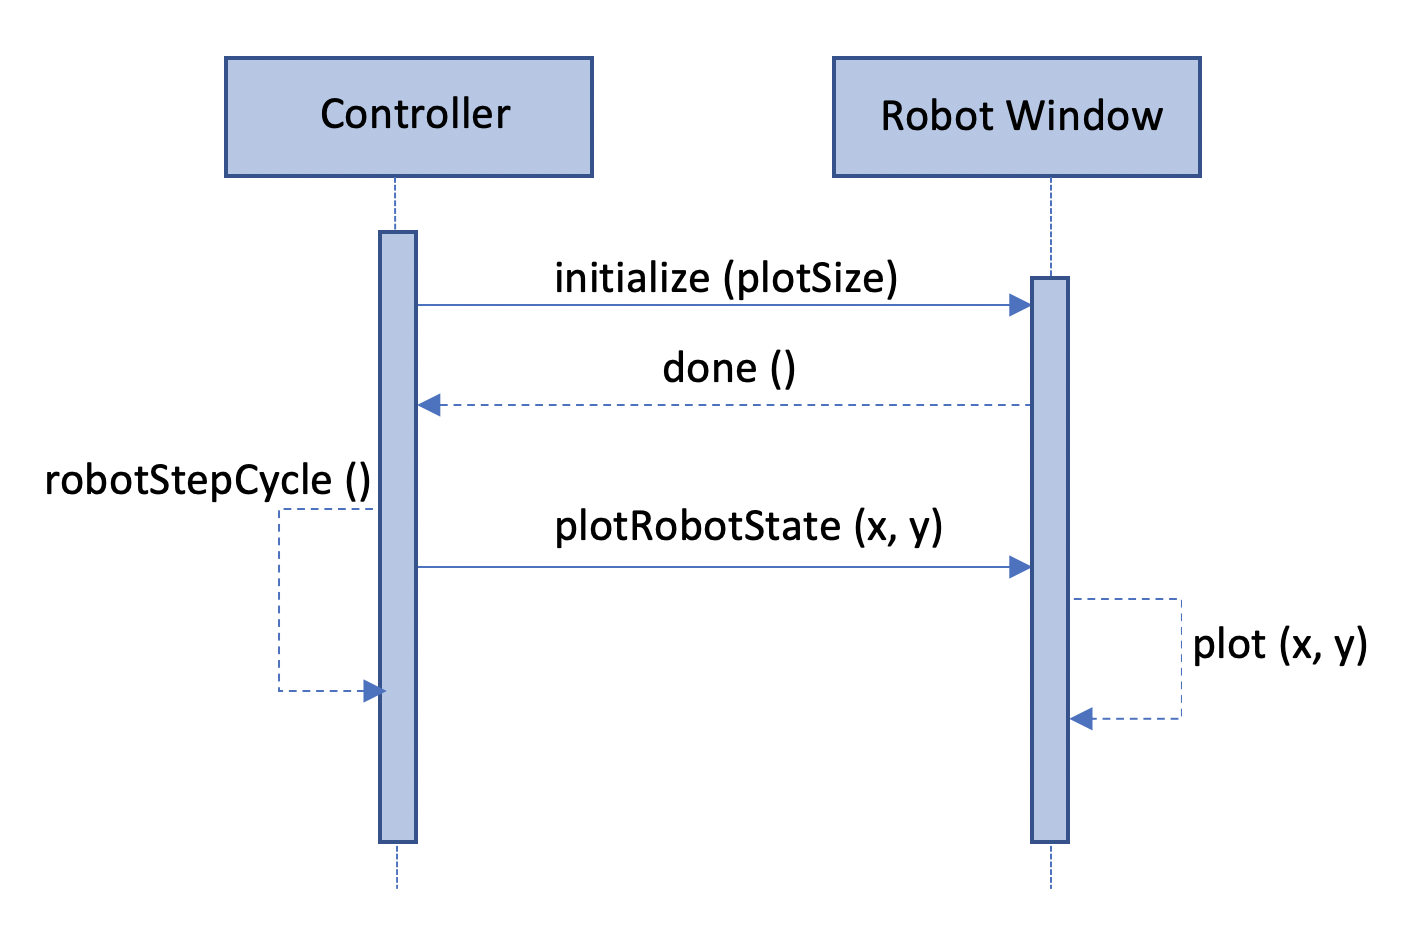
\includegraphics[width=\linewidth]{\images/chapter3/seq-diagram-plot.png}
  \caption{Sequence diagram for plotting robot positioning.}
  \label{fig:ch-3:seq-diagram-plot.png}
\end{figure}

Figure \ref{fig:ch-3:seq-diagram-plot.png} shows through a sequence diagram how the controller communicates with the robot window. First the controller sends an initialization command to the robot window together with some parameters such as the arena size. Once the simulation starts at each robot step the controller sends the robot positioning coordinates to the robot window which is in charge of plotting them. 

\begin{figure}[h!]
  \centering
  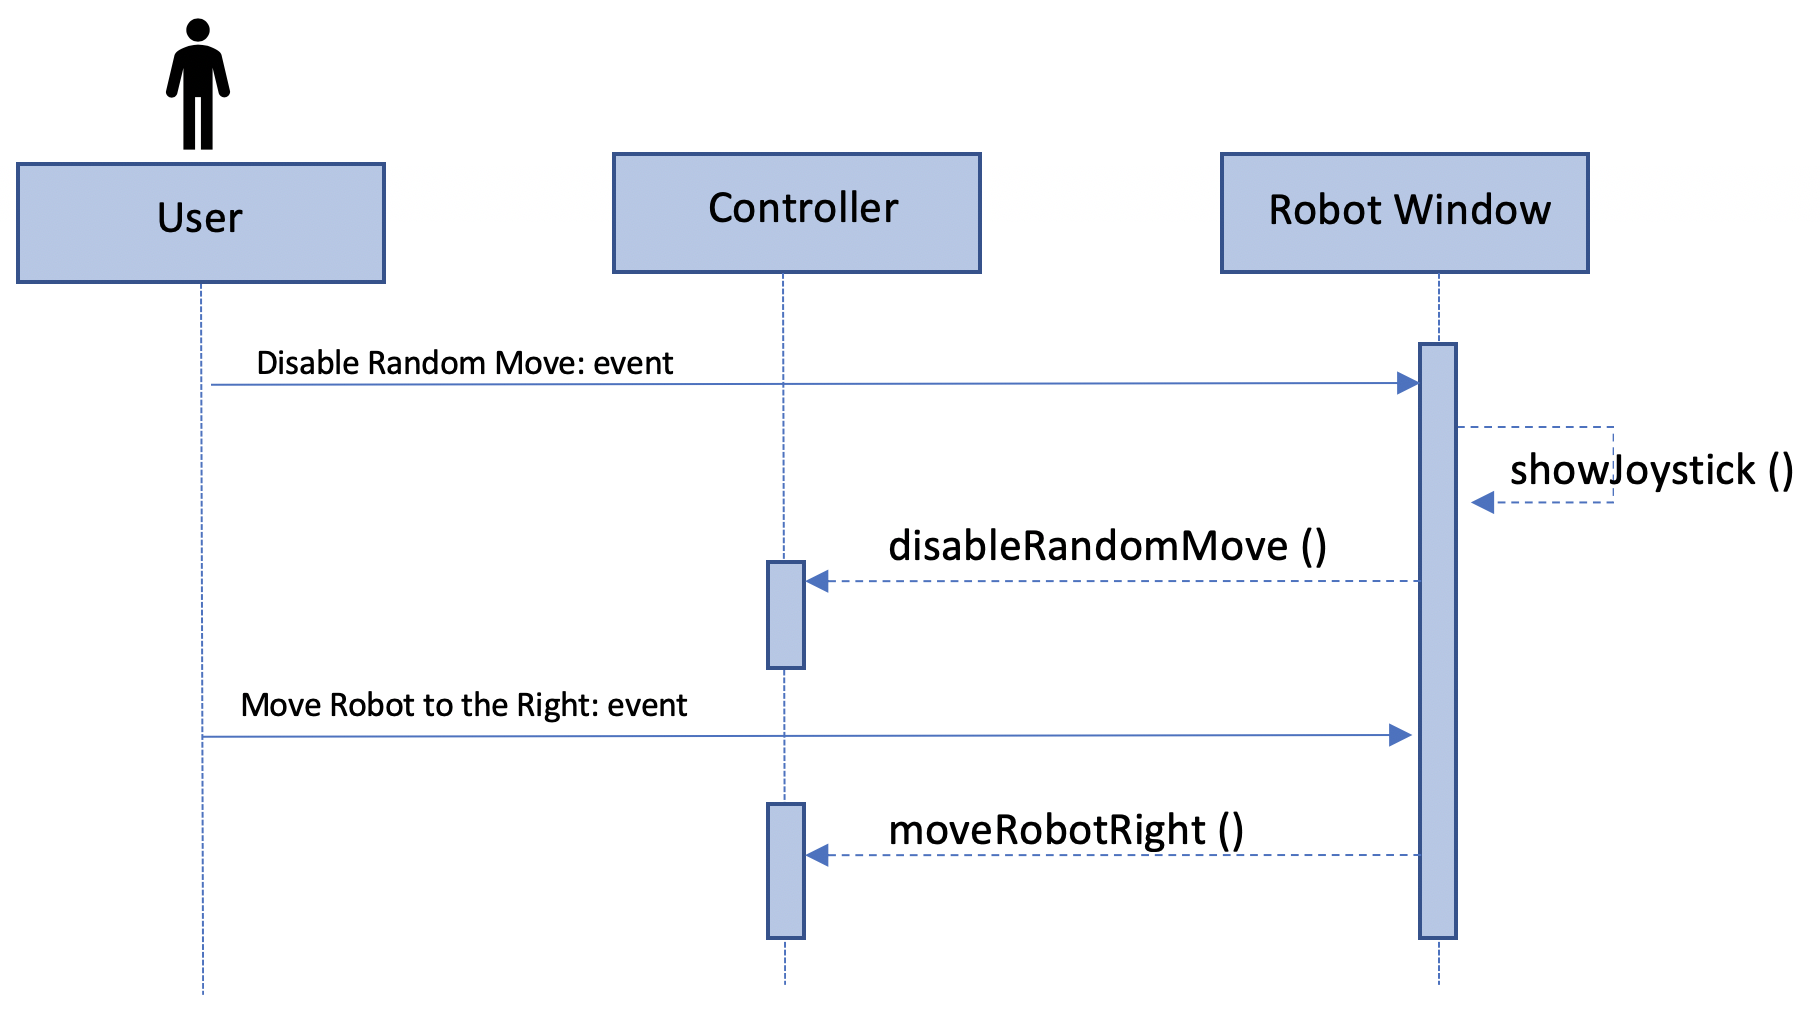
\includegraphics[width=\linewidth]{\images/chapter3/seq-diagram-movement.png}
  \caption{Sequence diagram for robot random movement deactivation.}
  \label{fig:ch-3:seq-diagram-movement}
\end{figure}

The random robot movement is disabled when the user clicks on the switch component. This is made through the robot window which afterwards sends a message to the robot controller to stop moving the robot. Additionally, a joystick is displayed to the user who has four possibilities: move the robot up, down, left or right. Once one of these options is selected the robot window sends a message to the controller with the desired movement to do, then the latter translates this action to the robot wheels actuators. This process is presented in figure \ref{fig:ch-3:seq-diagram-movement}. When the random robot movement is enabled again the controller is communicated about this action and starts moving the robot randomly.

This robot window offers some control over the robot in order to see the result of the experiments while running the simulation.

